% Backup slides
\appendix

% === B0a/b: Full headline figures ============================================

\begin{frame}[t]{Backup --- E1 headline figure (full-reprocess)}
  \begin{center}
    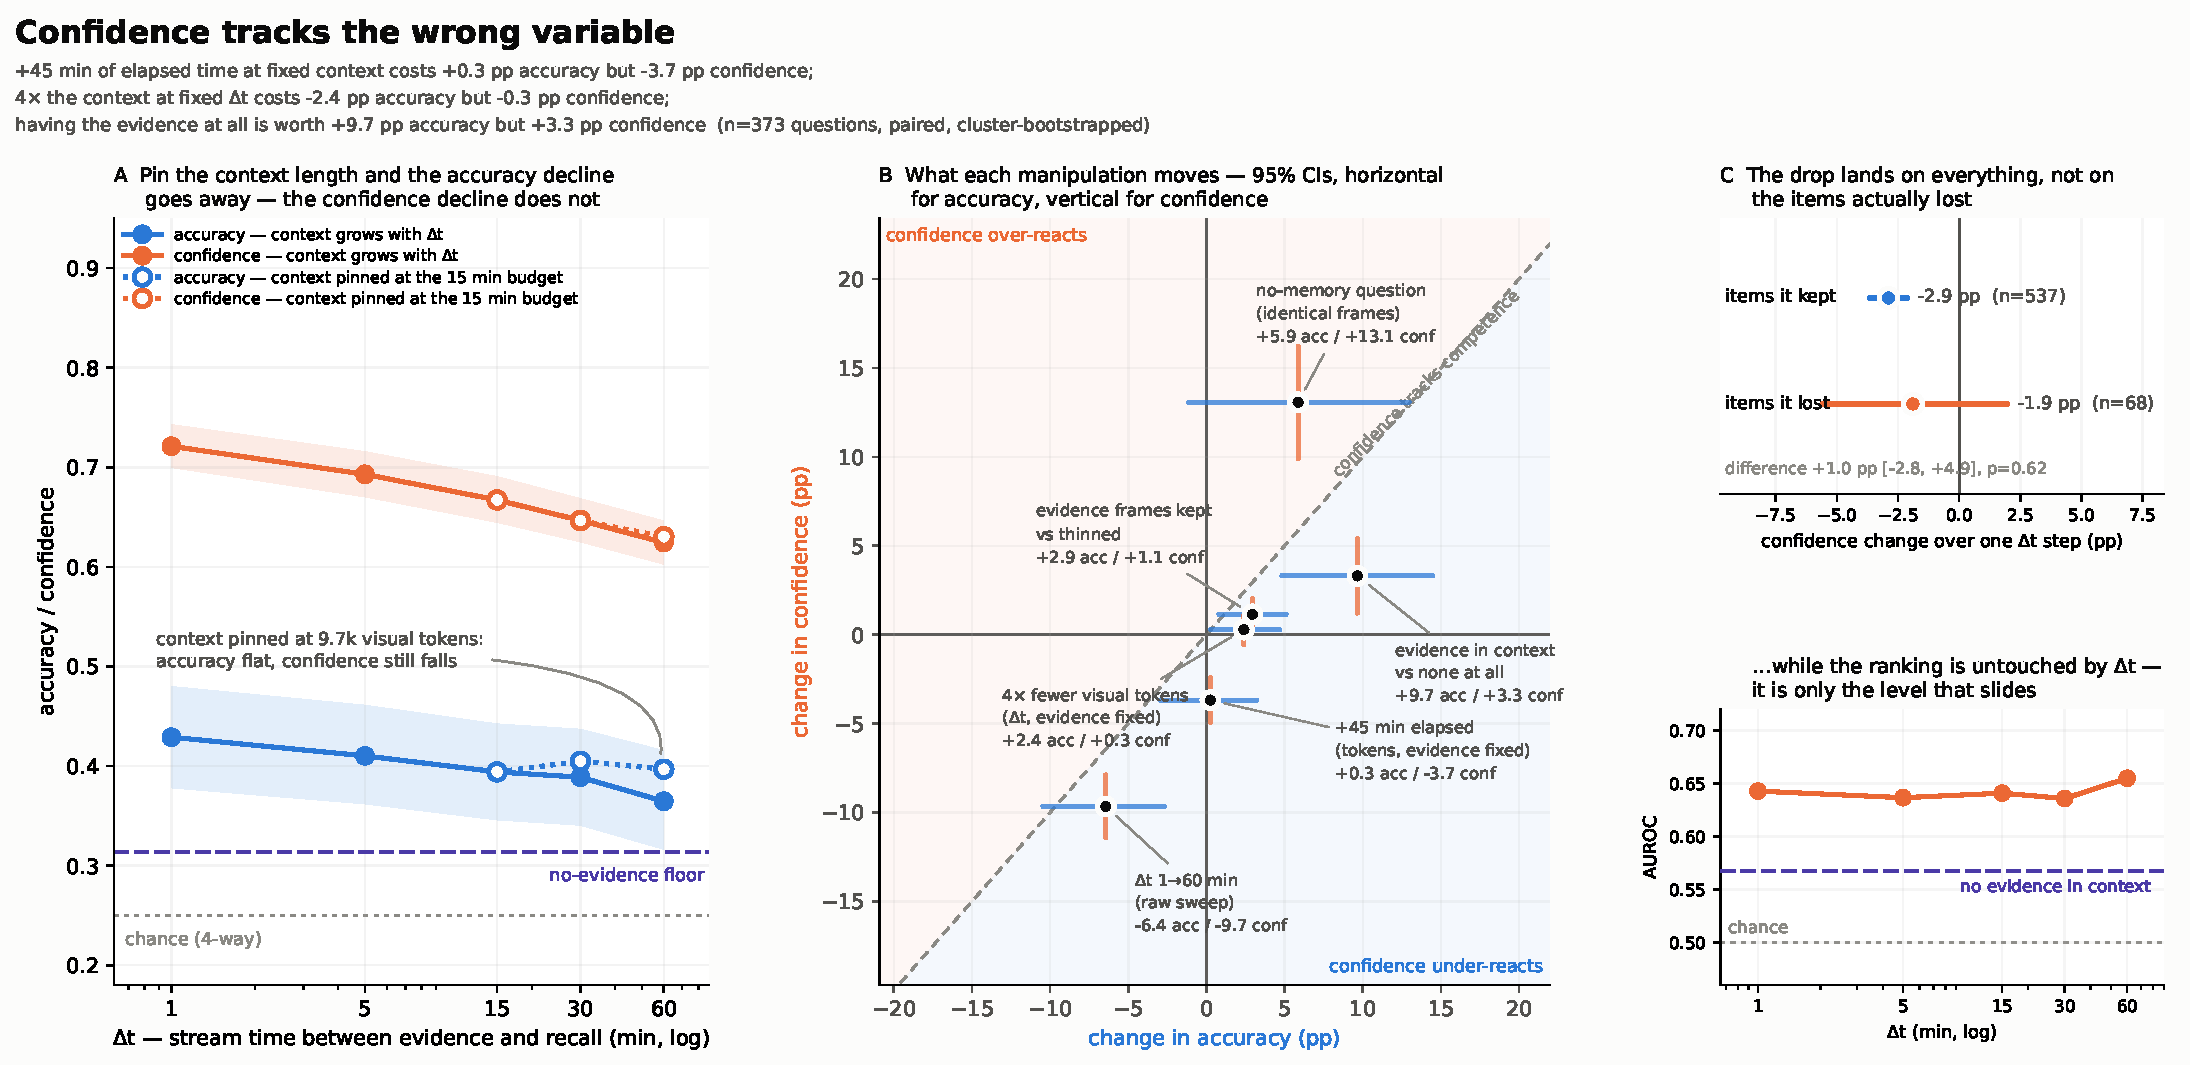
\includegraphics[width=\textwidth,height=0.85\textheight,keepaspectratio]{e1-full.pdf}
  \end{center}
\end{frame}

\begin{frame}[t]{Backup --- E2 headline figure (streaming KV cache)}
  \begin{center}
    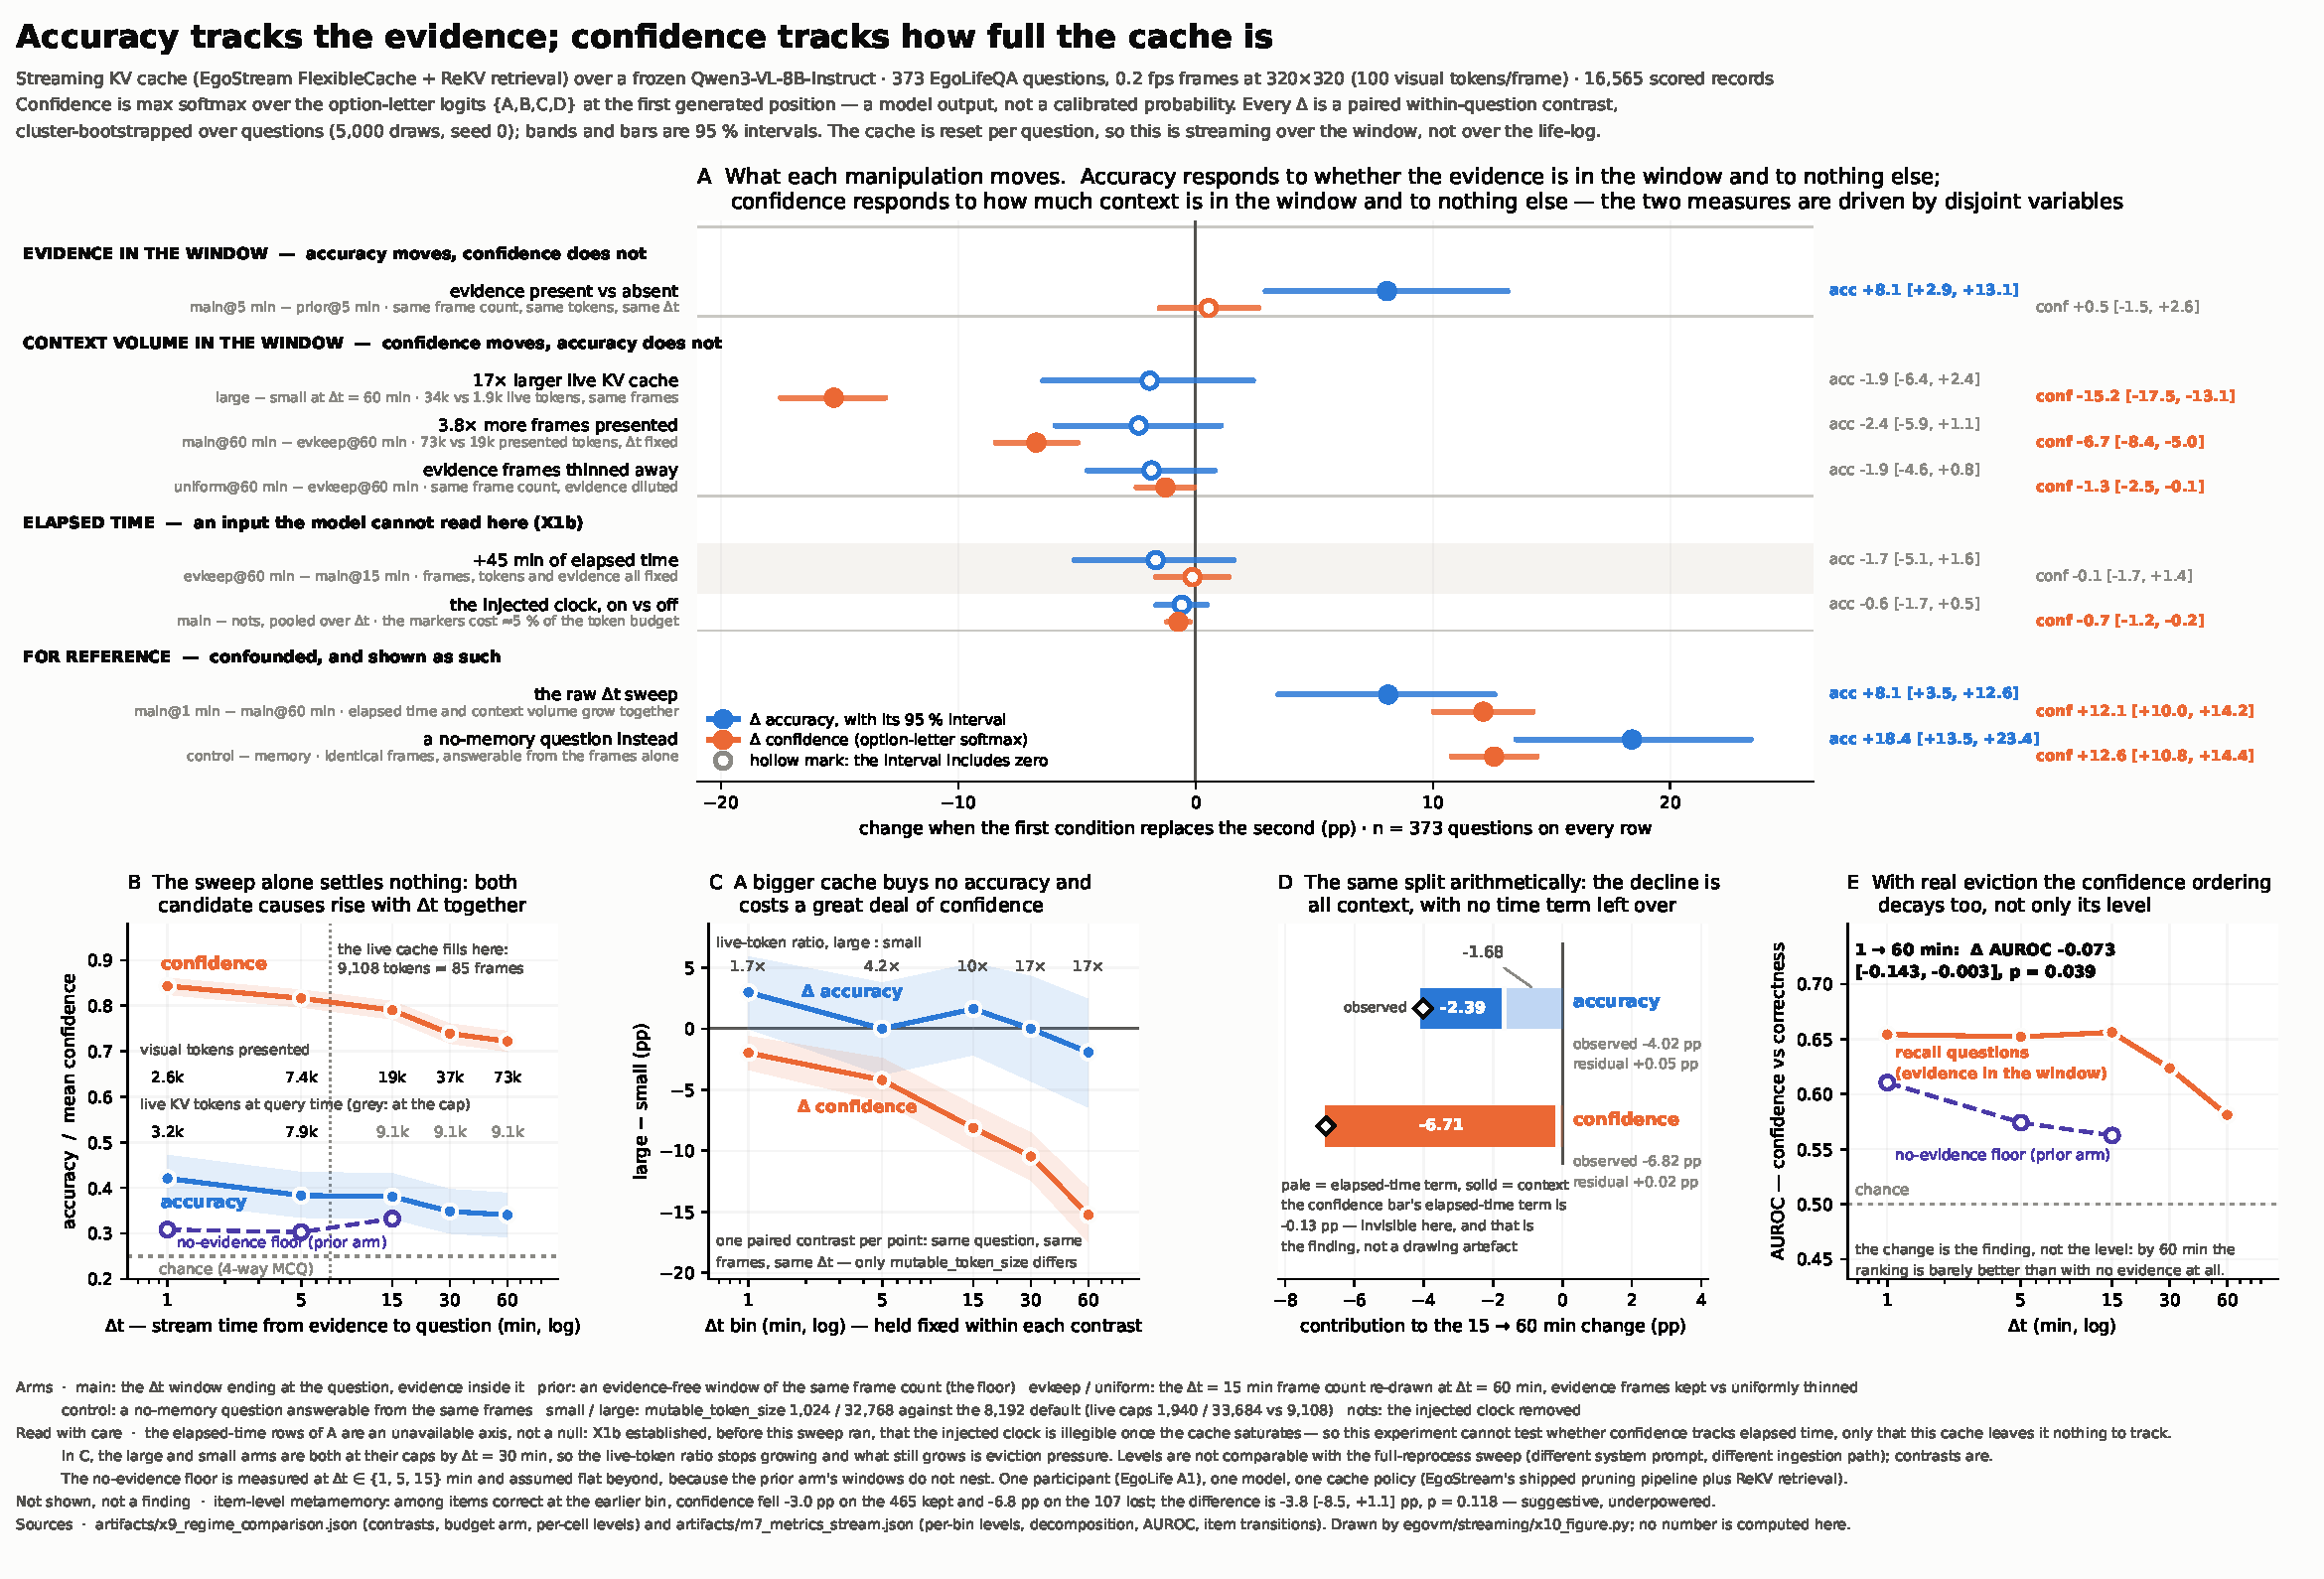
\includegraphics[width=\textwidth,height=0.85\textheight,keepaspectratio]{e2-full.pdf}
  \end{center}
\end{frame}

% === B1: Key definitions =====================================================

\begin{frame}[t]{Backup --- confidence probe definition and robustness}
  \begin{columns}[T]
    \begin{column}{0.48\textwidth}
      {\footnotesize\textbf{Definition.} $\mathrm{confidence} = \max_{L\in\{A,B,C,D\}} \mathrm{softmax}(z_L)$ at the first generated position, no text generated. Correctness is $\mathrm{argmax}$ vs gold. This is Tsvilodub et al.\ 2024 / EgoSAT Eq.~6.}
      \vskip0.5em
      {\footnotesize\textbf{Denominator.} Restricted to the four option letters. Mean mass on $\{$A,B,C,D$\}$: \MassEone\ (\Eone), \MassEtwo\ (\Etwo). Argmax disagreements: \textbf{\ArgmaxDisagree} records.}
      \vskip0.5em
      {\footnotesize\textbf{Denominator sensitivity.} Vocabulary-normalised softmax is inert except on \Etwo\ \texttt{evidence\_vs\_none}, where it gives \conf{\VocabEvidenceEtwo} --- driven by the off-letter tail (P4).}
    \end{column}
    \begin{column}{0.50\textwidth}
      {\footnotesize\textbf{Robustness.} AUROC is invariant to scalarisation:}
      \vskip0.3em
      \scriptsize
      \begin{tabular}{@{}lrr@{}}
        \toprule
        \thead{discriminator} & \thead{\Eone} & \thead{\Etwo} \\
        \midrule
        max-p, restricted & \AurocRestrEone & \AurocRestrEtwo \\
        max-p, vocab-normalised & \AurocVocabEone & \AurocVocabEtwo \\
        negative entropy & 0.6228 & \AurocEntropyEtwo \\
        margin (top1 $-$ top2) & 0.6254 & \AurocMarginEtwo \\
        \bottomrule
      \end{tabular}
      \vskip0.5em
      {\footnotesize\textbf{Option-letter bias.} \Eone\ predicts C on 43.5\,\%, \Etwo\ predicts B on 34.2\,\%, against near-uniform gold. Paired design cancels it. EgoSAT runs the cyclic-permutation check we do not.}
    \end{column}
  \end{columns}
  \source{\texttt{memo/CONFIDENCE-PROBE.md}}
\end{frame}

% === B2: Dataset curation ====================================================

\begin{frame}[t]{Backup --- dataset curation: 500 $\rightarrow$ 373 questions}
  \begin{columns}[T]
    \begin{column}{0.52\textwidth}
      \footnotesize
      \begin{tabular}{@{}p{3.6cm}rrl@{}}
        \toprule
        \thead{step} & \thead{in} & \thead{out} & \thead{reason} \\
        \midrule
        EgoLifeQA A1 (full) & 500 & --- & \\
        Drop TaskMaster & 500 & 437 & prospective \\
        Screen HabitInsight & 437 & 376 & no single anchor \\
        Evidence span $>$\,15\,min & 376 & 373 & ambiguous \dt \\
        \bottomrule
      \end{tabular}
      \vskip0.3em
      {\footnotesize EntityLog\,/\,EventRecall\,/\,RelationMap at 125\,/\,124\,/\,124. All 373 in every \dt\ bin and arm. Token-matched arms hold visual tokens exactly at the \dt\,=\,15\,min level.}
    \end{column}
    \begin{column}{0.45\textwidth}
      {\footnotesize\textbf{TaskMaster} (63): prospective, incompatible with retrospective \dt. 93.7\,\% require audio.}
      \vskip0.2em
      {\footnotesize\textbf{HabitInsight} (61): no single evidence event to anchor \dt. Scored separately.}
      \vskip0.2em
      {\footnotesize\textbf{Span exclusions} (3): q482 spans 50.7\,h. q189/q346 at 19/21\,min.}
      \vskip0.3em
      \claim{\scriptsize EgoLifeQA participant A1/Jake --- the only released participant. One model, one cache policy.}
    \end{column}
  \end{columns}
  \source{M1 \texttt{m1\_questions.py}, M4 \texttt{m4\_plan.py}.}
\end{frame}

% === B3: Self-use notes (not for presentation) ===============================

\begin{frame}[t]{Backup --- self-use: what is \emph{not} in these slides}
  \footnotesize
  \begin{enumerate}\setlength\itemsep{0.35em}
    \item \textbf{Cross-regime rotation.} Confidence driver swaps: elapsed time in \Eone\ (\conf{\EoneElapsedConf}), context volume in \Etwo\ (\conf{\EtwoFourxConf}). Differences exclude zero (\conf{\XregElapsedConf} and \conf{\XregFourxConf}). On evidence: \Eone\ gave \acc{\EoneEvidenceAcc}/\conf{\EoneEvidenceConf}; cross-regime $\Delta$confidence \conf{\XregEvidenceConf}.

    \item \textbf{Elapsed time is \emph{unavailable} in E2, not null.} EgoStream's image path has no native time markers; injected ones are unreadable once the cache saturates.

    \item \textbf{Item-level metamemory.} Suggestive, underpowered: \EtwoItemDiff, $p$ = \EtwoItemDiffP, on \EtwoItemLost\ lost items.

    \item \textbf{Original hypothesis rejected.} Widening gap absent both times (\Eone: \EoneGap, $p$ = \EoneGapP; \Etwo: \EtwoGap, $p$ = \EtwoGapP).

    \item \textbf{Cheapest follow-ups.} (a)~Strip timestamps from \Eone\ (\TimestripCost). (b)~Recalibrate on \texttt{live\_tokens} (free). (c)~Top-$k$ dump on \texttt{prior} for off-letter mass.
  \end{enumerate}
\end{frame}

\begin{frame}[t]{Backup --- scope conditions}
  \begin{itemize}\footnotesize\setlength\itemsep{0.4em}
    \item \textbf{Window, not life-log.} Each question resets the cache. No claim about 44\,h of history.
    \item \textbf{Evidence effect resolved at \dt\ $\leq$ 15 min only.} The floor is measured at every bin; by 30--60 min the contrast itself is within noise.
    \item \textbf{Levels not comparable across regimes.} \Etwo\ changes prompt and ingestion path. Contrasts are comparable.
    \item \textbf{Dynamic range $\sim$11\,pp.} Bin-1 accuracy \EtwoBinOneAcc\,\% against floor \EtwoFloorAcc\,\%.
    \item \textbf{One participant, one model, one cache policy.}
    \item \textbf{``Confidence'' is not a calibrated probability.} Report as ``option-letter softmax''.
  \end{itemize}
\end{frame}
